% 例 1：直角三角形 AC=3, BC=4, AB=5
\documentclass[tikz,border=4pt]{standalone}
\usepackage{ctex}
\usepackage{amsmath}
\begin{document}
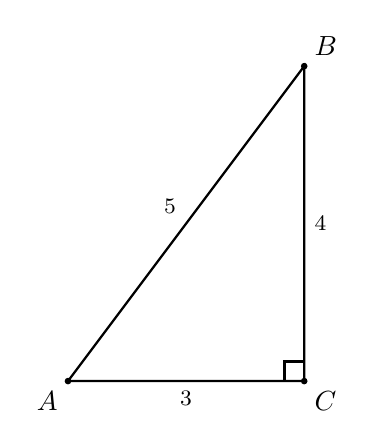
\begin{tikzpicture}[scale=1.0, thick]
  \coordinate (A) at (0,0);
  \coordinate (C) at (3,0);
  \coordinate (B) at (3,4);
  \draw (A) -- (C) -- (B) -- cycle;
  \draw (2.75,0) -- (2.75,0.25) -- (3,0.25);
  \fill (A) circle (1.2pt); \fill (B) circle (1.2pt); \fill (C) circle (1.2pt);
  \node[below left] at (A) {$A$};
  \node[below right] at (C) {$C$};
  \node[above right] at (B) {$B$};
  \node[below] at (1.5,0) {\footnotesize $3$};
  \node[right] at (3,2) {\footnotesize $4$};
  \node[above left] at (1.5,2) {\footnotesize $5$};
\end{tikzpicture}
\end{document}
